%First document, firstdocumentill.tex
\documentclass{amsart}
\usepackage{amssymb,latexsym}
\usepackage{graphicx}

\newtheorem{theorem}{Theorem}

\begin{document}
\title{A technical result\\ for congruences of finite lattices}  
\author{G. Gr\"{a}tzer} 
\address{Department of Mathematics\\
  University of Manitoba\\
  Winnipeg, MB R3T 2N2\\
  Canada}
\email[G. Gr\"atzer]{gratzer@me.com}
\urladdr[G. Gr\"atzer]{http://tinyurl.com/lej5g49}
\date{March 21, 2014}
\subjclass[2010]{Primary: 06B10.}
\keywords{finite lattice, congruence.}
\begin{abstract}
We present a technical result
for congruences on finite lattices.
\end{abstract}
\maketitle

\section{Introduction}\label{S:Introduction}%Section~\label{S:Introduction}
In some recent research, G. Cz\'edli
and I, see \cite{gC13} and \cite{GS13}, spent quite an effort
in proving that some equivalence relations 
on a planar semimodular lattice are congruences. 
The number of cases we had to consider
was dramatically cut by the following result.

\begin{theorem}\label{T:technical}%Theorem~\ref{T:technical}
Let $L$ be a finite lattice. 
Let $\delta$ be an equivalence relation on $L$
with intervals as equivalence classes.
Then $\delta$ is a congruence relation if{}f 
the following condition and its dual hold:
\begin{equation}\label{E:cover}%\eqref{E:cover}
\text{If $x$ is covered by $y,z \in L$ 
and $x \equiv y \pmod{\delta}$,
then $z \equiv y + z \pmod{\delta}$.}\tag{C${}_{+}$}
\end{equation}
\end{theorem}

\begin{figure}[hbt]
\centerline{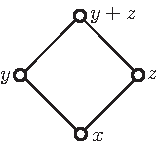
\includegraphics{covers}}
\caption{Theorem~\ref{T:technical} illustrated}\label{T:Theorem}
\end{figure}

\section{The proof}\label{Proof}%Section~\label{S:Proof}
We prove the join-substitution property:  
if $x \leq y$ and $x \equiv y \pmod{\delta}$, then
\begin{equation}\label{E:Cjoin}%\eqref{E:Cjoin}
x + z \equiv y + z \pmod{\delta}.
\end{equation}
Let $U = [x, y+ z]$.
We induct on length\,$U$, the length of $U$.  

Let $I=[y_1,y+ z]$ and $J=[z_1,y+ z]$. 
Then length\,$I$ and length\,$J  < $ length\,$U$. 
Hence, the induction hypothesis applies to $I$ 
and $\delta\rceil I$, and we obtain that 
$w \equiv y+ w \pmod{\delta}$. 
By the transitivity of $\delta$, we conclude that 
\begin{equation}\label{E:three}%\eqref{E:three}
z_1 \equiv y+ w \pmod{\delta}.
\end{equation}
Therefore, applying the induction hypothesis to $J$ 
and $\delta \rceil J$, we conclude \eqref{E:Cjoin}.

\begin{thebibliography}{9}
\bibitem{gC13}%G. Cz\'edli~\cite{gC13}
G. Cz\'edli,
\emph{Patch extensions and trajectory colorings of slim
rectangular lattices.}
Algebra Universalis. 

\bibitem{GS13}%G. Gr\"atzer \cite{GS13}
G. Gr\"atzer, 
\emph{Congruences of fork extensions of lattices.}
Acta Sci. Math. (Szeged). 
\end{thebibliography}
\end{document}